\chapter{Contributions}

While Julia produces usually faster code than other languages at the same abstraction level for numerical application, the true power of the language is only shown when the programmer writes the code following a couple performance tips listed on the official documentation. One of the most commonly occurring mistake that results suboptimal code is the high number of automatic memory allocations that leads to more frequent calls to garbage collector, and in other words, it wastes resources. Therefore in the following presentation of the programming-related contributions we will highlight the memory-efficiency at the evaluation of the created code base.

\section{FunctionOperators package}

As we have seen so far in the descriptions of the algorithms, operations very often are expressed as a multiplication a matrix-like entity and a vector or matrix. That notation is particularly convenient as it allows using the same set of mathematical tools as we have for matrices, while allows extension of the capabilities of the conventional linear mapping defined as a matrix-vector multiplication. In practice that means that we would like to combine the flexibility of functions with the power of tools designed for matrices, so many times the best option is to define the operation we want to perform as a function, and then wrap this function in an object that acts like a matrix and therefore it is compatible for instance with iterative solvers like the conjugate gradient method. Also it is desirable to add an "backward" operation, also defined by a function, to that wrapper object, that defines what should the solver do when it wants to use the adjoint of the operator.

Being driven by mostly scientists, the Julia community has already developed some packages that helps keeping the code structurally and visually similar to the abstract mathematical notation; nevertheless, none of these were completely satisfying. In particular, there are three relatively popular packages that have such functionality, but all of them some drawbacks:
\begin{itemize}
    \item LinearOperators.jl~\cite{noauthor_juliasmoothoptimizerslinearoperatorsjl_2020} and LinearMaps.jl~\cite{jutho_jutholinearmapsjl_2020} aims to provide almost all features of general matrices, but this design choice restricts the possible inputs to vectors.
    \item AbstractOperators.jl~\cite{noauthor_kul-forbesabstractoperatorsjl_2020} is a fairly new package that overcomes this limitation and provides a relatively large range of features, mostly in the form of predefined operators for the most common operations such as DFT, convolution, finite differences etc. It is also memory effective, preallocating a buffers when two operators are composed (that corresponds to the matrix-matrix multiplication) and it reuses this buffer later avoiding unnecessary memory allocations. Unfortunately, this optimization makes it impossible to accept on GPU arrays that makes unfavorable for large-scale applications.
\end{itemize}

As Julia is designed to be very extendable, it is always a feasible option to develop a new package that fits the specific problem. After reviewing the code of the mentioned packages, we came to the conclusion that the design choices of these packages doen't allow addition of features we desired, without breaking the already existing features, we decided to implement a package that fits better the image CS-MRI reconstruction framework. The developed package is named FunctionOperators.jl and it is already published to the central Julia package repository. Being just after the initial phase, the package supports only the most basic features, but the design of the interface and the efficient implementation lets the user build arbitrarily complex composite operators without having any computation penalty compared to the implementation with pure functions. As of today, the already implemented features if the package are the following:
\begin{itemize}
    \item Construction from a function with one argument that defines "forward" operation. When the constructed FunctionOperator is being multiplied with a vector/matrix of the \textit{proper} size, this function is called on the given vector/matrix. The size of the \textit{proper} input and expected output is a mandatory argument of the constructor of FunctionOperator, and any input with a mismatching size is rejected, and it after the multiplication the size of the output is also checked against the output size specified at construction. E.g. `Op = FunctionOperator(forw = x -> fft(x)); y = Op * x` calculates the FFT of x and stores in y.
    \item Construction from two functions both accepting one argument. These functions define the "forward" and the "backward" operations. In contrast to the "forward" function, the "backward" function is called when adjoint of the FunctionOperator is requested. E.g. `Op = FunctionOperator(forw = x -> fft(x), backw = x -> ifft(x)); y = Op' * x` calculates the inverse FFT of x and stores in y.
    \item These "forward" and "backward" functions also can accept two arguments. In that case, the second argument is the input of the operation, and the functions are expected to store the result of the operation in the first argument. This feature is advantageous if one wants to optimize the number of memory allocations. E.g. `Op = FunctionOperator(forw = (b,x) -> b .= x .* 2); mul!(y, Op, x)` multiplies x elementwise with two and stores the result in y without allocating an intermediate array.
    \item Composition of FunctionOperators by multiplication (that means composition of the "forward" functions), addition and substraction (these adds/substracts the output of the operations). E.g. considering `Op1 = FunctionOperator(forw = x -> fft(x)); Op2 = FunctionOperator(forw = (b,x) -> b .= x .* 2);` the output of `Op1 * Op2 * x` is the same as fft(x .* 2)
    \item Composition of FunctionOperators with UniformScaling object from LinearAlgebra standard library. This UniformScaling operator corresponds to the identity matrix. E.g. we can define the MR acquisition operator $\mathcal{A}$ as a FunctionOperator, and then we can define the CG operator in algorithm~\ref{alg:al-cg} as $\mathcal{A}' * \mathcal{A} + \delta_1 I$ (it is not the abstract mathematical notation, but a valid Julia expression!) and then we can pass it to a a solver (IterativeSolver.jl has, for example, CG solver that uses duck-typing, so it requires only that the multiplication must be implemented on the object passed as argument).
    \item Adjoint of composit FunctionOperators: If the FunctionOperator is a composition of other FunctionOperators, then the adjoint is defined as the composition of adjoints of the member FunctionOperators, in the reverse order. E.g., let us recall the decomposition of the acquisition operator $\mathcal{A} = \Omega \mathcal{FC}$. Now look on it on the other way around: we have $\Omega, \mathcal{F}$ and $\mathcal{C}$ already created as FunctionOperators, and we create the acquisition operator as the composition of them: $\mathcal{A} = \Omega * \mathcal{F * C}$. Then $\mathbf{A}' * x$ would do the same as $\mathcal{C' * F'} * \Omega' * x$.
\end{itemize}

Under the hood, the most important property of the package that it uses the least amount of memory possible by deferring the allocation of buffers as much as possible and also by maintaining a smart global pool that stores the already allocated buffers. These buffers are only needed to store intermediate results, and therefore they are safe to reuse in different FunctionOperators provided that they are on the same thread. But the user don't need to worry about that criterion since this case is handled automatically, making FunctionOperators a thread-safe package (assuming that the user builds the operators from thread-safe "forward" and "backward" functions). This memory effective implementation makes FunctionOperators a truly unique as other packages are all more or less suboptimal in this sense.

As an extra (yet experimental) feature, FunctionOperators package provides a macro that automatically optimizes loops by cutting down the number unnecessary memory allocations. To achieve this the macro uses the advanced code generation features that produces code before the compilation of the program, but after the parser has built the abstract syntax tree and deduced the type of variables; therefore, heavy optimizations can be performed behind the scenes using macros and generated functions. %Fig.~\ref{} shows three versions of the same code fragment: one is a readable version that resembles the mathematical formulation, the other is a memory-wise optimal, but much less readable code, and the third one show the usage of the macro that reduces the amount of allocated memory by $~70\%$.

Following the guidelines of the Julia community for package development, the code is thoroughly tested using unit tests, and has a clean documentation that contains a notebook with an example for almost all features. The coverage of unit tests are measured by \url{codecov.io}, and it reported that the $94\%$ of the code is covered. This report, however, underestimates the coverage as it fails to detect the covered lines in case of tests checking the functions that prints to console. The code of the package is uploaded to \url{https://github.com/hakkelt/FunctionOperators.jl}, and the documentation is available at \url{https://hakkelt.github.io/FunctionOperators.jl/latest/}.

\section{Implementation of Sparse+Low Rank algorithms}

After the careful examination of both the publication and the reference Matlab implementation, we created an efficient Julia version for each of these algorithms. As the implementation was done at the same time as the FunctionOperators was developed, it was a natural choice to benchmark the newly developed package against the other similar packages on these algorithms. The contribution of this part of the project is two-fold: First, it extends the currently small code base of MRI-related algorithms in Julia, helping the fast growing group of scientists choosing to prototype their research algorithms in Julia. Second, it might also help those who needs guidance in picking the right package, especially because currently no other comparison is available to see the difference between LinearMaps.jl and AbstractOperators.jl.

The result of the benchmarking is available in table~\ref{tab:lin_fessler} and the Jupyter notebooks holding both the benchmarking code, the documentation, and the results are available at \url{https://github.com/hakkelt/reproduce-l-s-dynamic-mri-julia}
In comparison to the Matlab implementation, the results are somewhat mixed since Julia outperformed Matlab in case of the improved AL scheme (the speedup here was ~2x) and in case of proximal methods for the non-Cartesian dataset (with 2-3.5x speedup). On the other hand, Matlab produced faster code for the other cases. This results underlines the fact that merely switching the language to Julia not necessarily results in increased speed automatically. A possible explanation is that we missed some hidden optimization tricks deeply buried in the Matlab code (which was well optimized indeed, and very hard to read---it required a fair amount of time from us to understand how is it connected to the theory described in the paper). Another possible factor is that Matlab uses some proprietary C and fortran libraries that have slightly better performance compared to the open source options bundled with Julia by default.

Furthermore, the comparison of different Julia implementations revealed that the three package have very similar running time and they differ mostly in the memory allocated, LinearMaps.jl having the largest memory demand (as it was expected from the implementation that allocates and releases buffers in each iteration again and again in our case), and FunctionOperators being better by a small margin. We also tested the automatic optimization macro mentioned above, and the benchmarks showed that it reached almost optimal memory usage, reducing the size of net allocations by $~70\%$ on average, compared to the $~80\%$ reduction achieved by the tedious process of manual optimization.

\begin{table}[]
\footnotesize
\begin{tabular}{|p{0.1\linewidth}|p{0.18\linewidth}p{0.18\linewidth}p{0.18\linewidth}p{0.18\linewidth}|}
\hline
algorithm \textbackslash data set & PINCAT & Multicoil cardiac cine MRI & Multicoil cardiac perfusion MRI & Multicoil abdominal dce MRI \\ \hline
\multicolumn{1}{|c|}{} & \multicolumn{4}{c|}{Matlab} \\
AL-CG & 16.8 s & 49.0 s & 19.9 s & - \\
AL-2 & 17.8 s & 55.3 s & 27.5 s & - \\
ISTA & 1.7 s & 5.5 s & 2.3 s & 141.8 s \\
FISTA & 2.4 s & 7.6 s & 3.1 s & 256.7 s \\
POGM & 1.8 s & 5.8 s & 2.3 s & 140.0 s \\ \hline
\multicolumn{1}{|c|}{} & \multicolumn{4}{c|}{LinearMaps} \\
AL-CG & 28.4 s, 11.26 GiB & 80.8 s, 31.08 GiB & 33.8 s, 12.95 GiB & - \\
AL-2 & 9.8 s, 6.22 GiB & 28.4 s, 17.56 GiB & 11.0 s, 7.32 GiB & - \\
ISTA & 6.0 s, 627.71 MiB & 19.6 s, 1.36 GiB & 6.8 s, 582.06 MiB & 72.7 s, 2.18 GiB \\
FISTA & 6.2 s, 627.71 MiB & 16.5 s, 1.36 GiB & 6.8 s, 582.06 MiB & 73.2 s, 2.18 GiB \\
POGM & 6.3 s, 677.71 MiB & 16.8 s, 1.45 GiB & 6.8 s, 622.06 MiB & 72.6 s, 2.42 GiB \\ \hline
\multicolumn{1}{|c|}{} & \multicolumn{4}{c|}{AbstractOperators} \\
AL-CG & 28.7 s, 678.06 MiB & 76.1 s, 1.45 GiB & 32.1 s, 622.41 MiB & - \\
AL-2 & 9.0 s, 1.14 GiB & 23.3 s, 2.93 GiB & 10.2 s, 1.22 GiB & - \\
ISTA & 6.4 s, 627.68 MiB & 16.4 s, 1.36 GiB & 7.3 s, 582.03 MiB & 72.8 s, 2.18 GiB \\
FISTA & 6.5 s, 627.68 MiB & 16.3 s, 1.36 GiB & 7.3 s, 582.03 MiB & 72.0 s, 2.18 GiB \\
POGM & 6.6 s, 677.68 MiB & 16.5 s, 1.45 GiB & 7.0 s, 622.03 MiB & 73.9 s, 2.42 GiB \\ \hline
\multicolumn{1}{|c|}{} & \multicolumn{4}{c|}{FunctionOperators naive} \\
AL-CG & 30.6 s, 2.90 GiB & 79.4 s, 6.14 GiB & 33.3 s, 2.43 GiB & - \\
AL-2 & 11.6 s, 12.20 GiB & 32.0 s, 33.17 GiB & 13.1 s, 13.82 GiB & - \\
ISTA & 6.8 s, 3.40 GiB & 18.1 s, 8.67 GiB & 7.6 s, 3.62 GiB & 72.7 s, 6.71 GiB \\
FISTA & 6.9 s, 3.40 GiB & 17.6 s, 8.67 GiB & 7.5 s, 3.62 GiB & 74.9 s, 6.71 GiB \\
POGM & 6.9 s, 3.45 GiB & 17.8 s, 8.77 GiB & 7.5 s, 3.65 GiB & 73.741 s, 6.96 GiB \\ \hline
\multicolumn{1}{|c|}{} & \multicolumn{4}{c|}{functionOperators optimized} \\
AL-CG & 27.0 s, 640.69 MiB & 76.2 s, 1.38 GiB & 33.0 s, 592.54 MiB & - \\
AL-2 & 8.6 s, 1.04 GiB & 22.7 s, 2.65 GiB & 10.0 s, 1.11 GiB & - \\
ISTA & 6.1 s, 627.79 MiB & 16.6 s, 1.36 GiB & 7.6 s, 582.14 MiB & 75.1 s, 2.18 GiB \\
FISTA & 6.1 s, 627.79 MiB & 16.5 s, 1.36 GiB & 7.9 s, 582.14 MiB & 73.8 s, 2.18 GiB \\
POGM & 6.3 s, 677.79 MiB & 16.747 s, 1.45 GiB & 7.079 s, 622.14 MiB & 73.6 s, 2.42 GiB \\ \hline
\multicolumn{1}{|c|}{} & \multicolumn{4}{c|}{FunctionOperators pretty} \\
AL-CG & 28.0 s, 741.02 MiB & 75.1 s, 1.57 GiB & 30.7 s, 662.87 MiB & - \\
AL-2 & 8.4 s, 1.26 GiB & 21.8 s, 3.26 GiB & 9.3 s, 1.36 GiB & - \\
ISTA & 6.3 s, 1.05 GiB & 16.4 s, 2.49 GiB & 6.9 s, 1.04 GiB & 73.5 s, 3.03 GiB \\
FISTA & 6.3 s, 1.05 GiB & 16.3 s, 2.49 GiB & 6.9 s, 1.04 GiB & 72.2 s, 3.03 GiB \\
POGM & 6.4 s, 1.10 GiB & 16.5 s, 2.58 GiB & 6.9 s, 1.08 GiB & 74.5 s, 3.28 GiB \\ \hline
\end{tabular}
\caption{Benchmarking on different datasets performing reconstruction via proximity and augmented Lagrangian methods descirbed in~\cite{lin_efficient_2019}. "FunctionOperators naive" is an implementation with minimal manual optimizations, "FunctionOperators optimized" is a manually optimized version, and ""FunctionOperators pretty" is exactly same as the "naive" version except that our automatic automatic optimizer macro is called on the code.}
\label{tab:lin_fessler}
\end{table}

\section{Implementation of Multiscale Decomposition}

\subsection{NUFFT}

\subsection{MSLR Algorithm}

%\subsection{Optimization possibilities}
%\begin{enumerate}
%    \item Batch-processing: compute NUFFT of all channels at once
%    \item Parallelization:
%    \begin{enumerate}
%        \item NUFFT
%        \item Algorithm
%    \end{enumerate}
%    \item GPU-specific optimizations:
%    \begin{enumerate}
%        \item Blocking operator might cause CPU bottleneck
%    \end{enumerate}
%\end{enumerate}

%\subsection{Parallelization Solution}
%Details how I made the code run parallel

\begin{figure}
    \centering
    \begin{minipage}{0.48\linewidth}
        \centering
        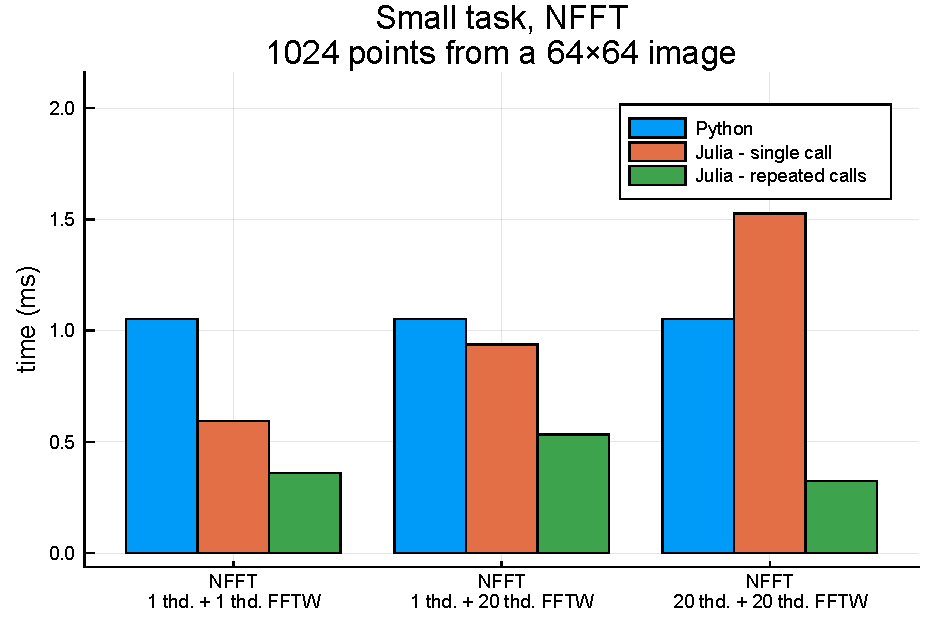
\includegraphics[width=\linewidth]{images/nfft_small_forw.pdf}
        \label{fig:nfft_small_forw}
    \end{minipage}
    \begin{minipage}{0.48\linewidth}
        \centering
        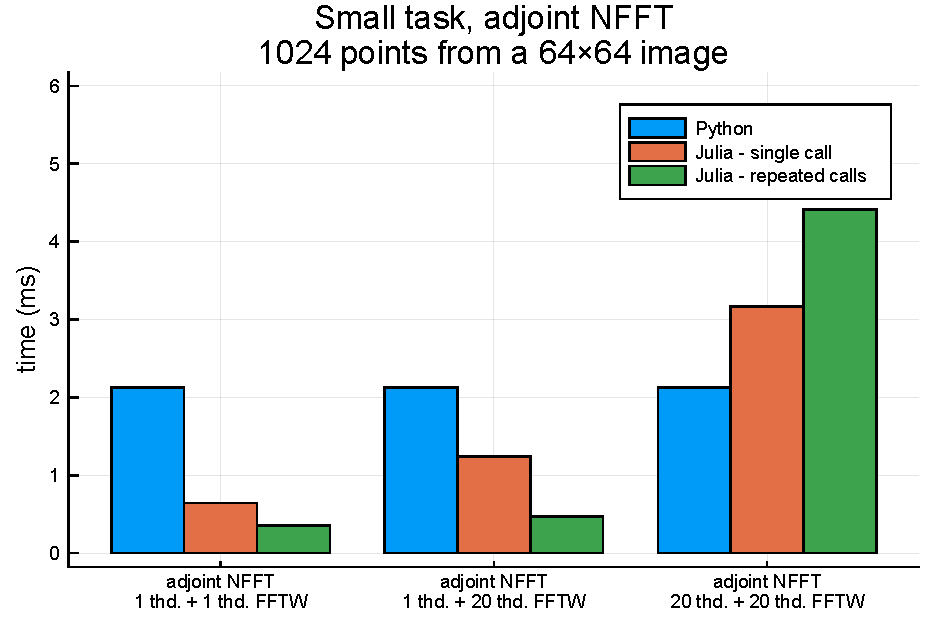
\includegraphics[width=\linewidth]{images/nfft_small_backw.pdf}
        \label{fig:nfft_small_backw}
    \end{minipage}
    \caption{\textbf{Comparison of running time} between the Python implementation in SigPy package (blue), and the Julia implementations (orange: initialization and computation, green: computation only) at different threading settings. (Note that the Python implementation does not implement multithreading, and hence the height of the three blue bar is the same.) \textbf{For small images, single threaded Julia version is the fastest.}}
    \label{fig:nfft_small}
\end{figure}


\begin{figure}
    \centering
    \begin{minipage}{0.48\linewidth}
        \centering
        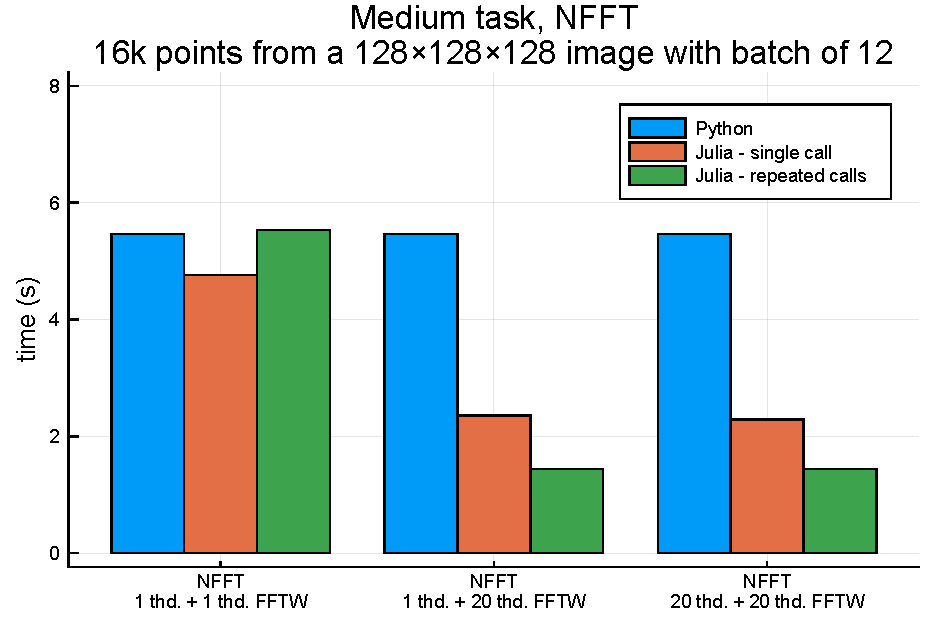
\includegraphics[width=\linewidth]{images/nfft_medium_forw.pdf}
        \label{fig:nfft_medium_forw}
    \end{minipage}
    \begin{minipage}{0.48\linewidth}
        \centering
        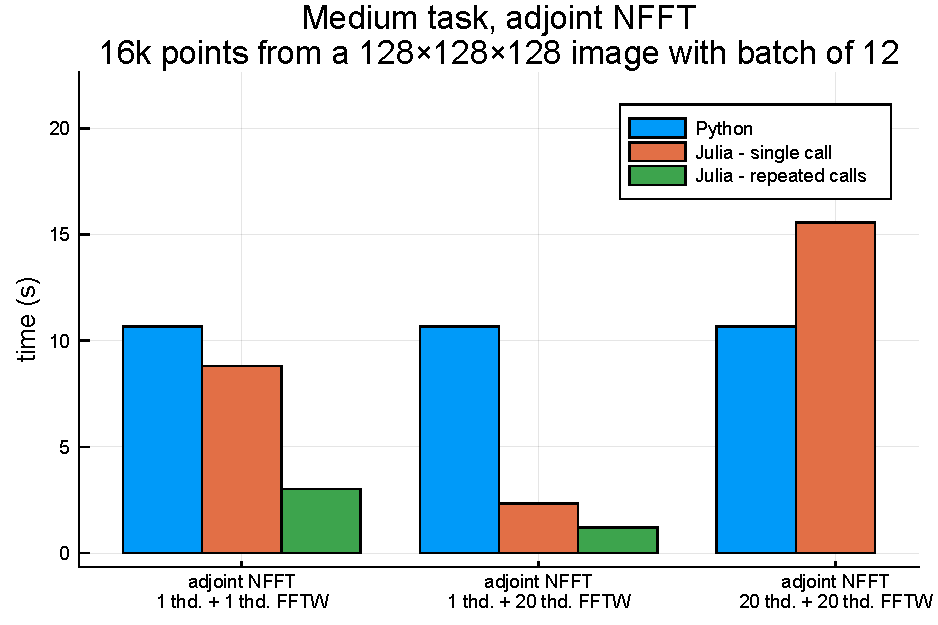
\includegraphics[width=\linewidth]{images/nfft_medium_backw.pdf}
        \label{fig:nfft_medium_backw}
    \end{minipage}
    \caption{\textbf{Comparison of running time} between the Python implementation in SigPy package (blue), and the Julia implementations (orange: initialization and computation, green: computation only) at different threading settings. (Note that the Python implementation does not implement multithreading, and hence the height of the three blue bar is the same.) \textbf{For small images, single threaded Julia version is the fastest.}}
    \label{fig:nfft_medium}
\end{figure}

\begin{figure}
    \centering
    \begin{minipage}{0.48\linewidth}
        \centering
        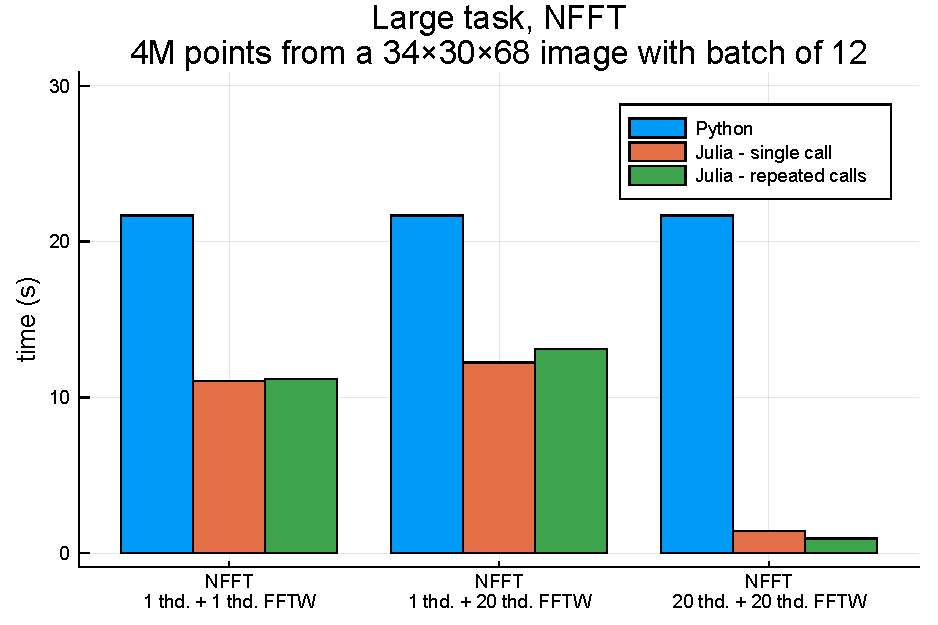
\includegraphics[width=\linewidth]{images/nfft_large_forw.pdf}
        \label{fig:nfft_large_forw}
    \end{minipage}
    \begin{minipage}{0.48\linewidth}
        \centering
        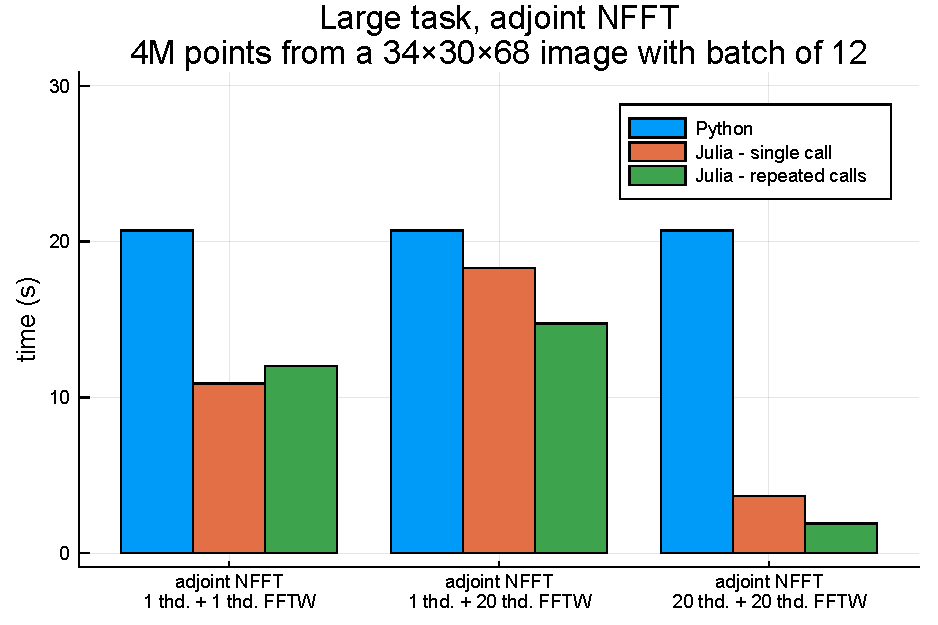
\includegraphics[width=\linewidth]{images/nfft_large_backw.pdf}
        \label{fig:nfft_large_backw}
    \end{minipage}
    \caption{\textbf{Comparison of running time} between the Python implementation in SigPy package (blue), and the Julia implementations (orange: initialization and computation, green: computation only) at different threading settings. (Note that the Python implementation does not implement multithreading, and hence the height of the three blue bar is the same.) \textbf{For small images, single threaded Julia version is the fastest.}}
    \label{fig:nfft_large}
\end{figure}

\begin{figure}
    \centering
    \begin{minipage}{0.48\linewidth}
        \centering
        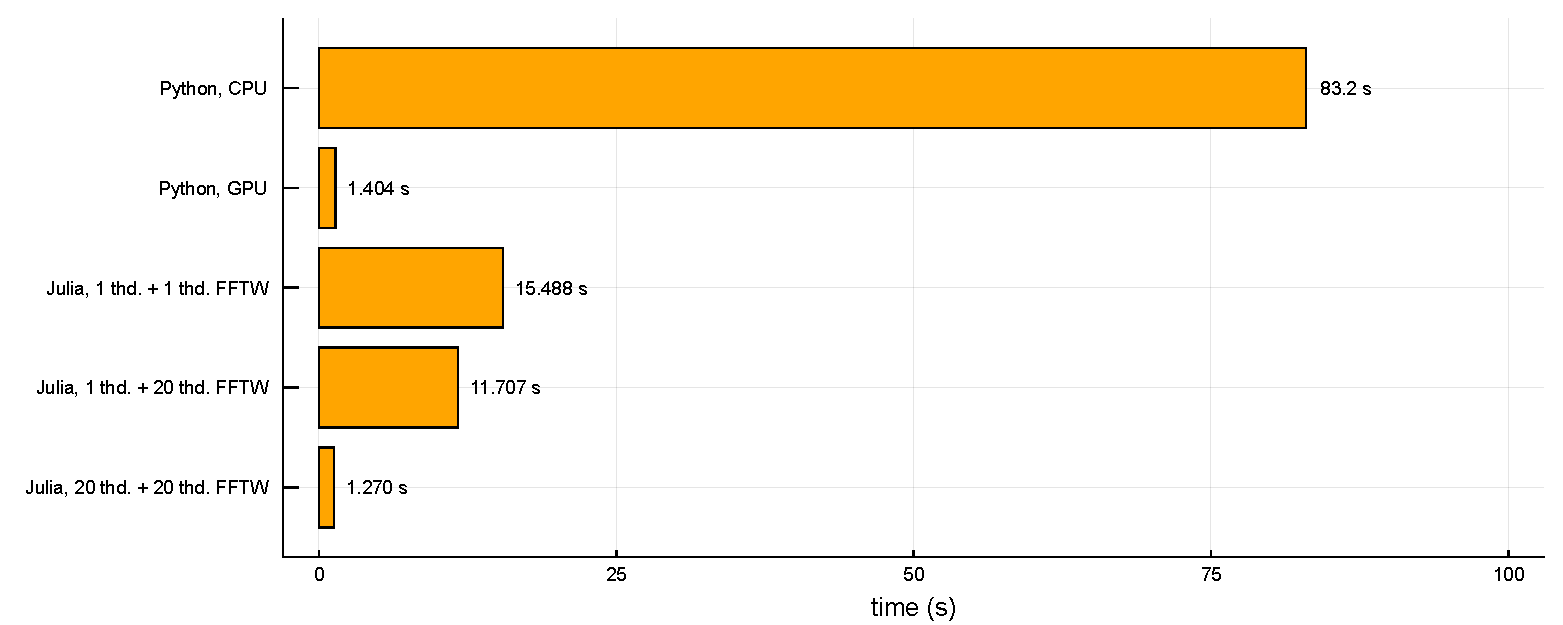
\includegraphics[width=\linewidth]{images/gridding_recon_speed.pdf}
        \label{fig:gridding_recon_speed}
    \end{minipage}
    \begin{minipage}{0.48\linewidth}
        \centering
        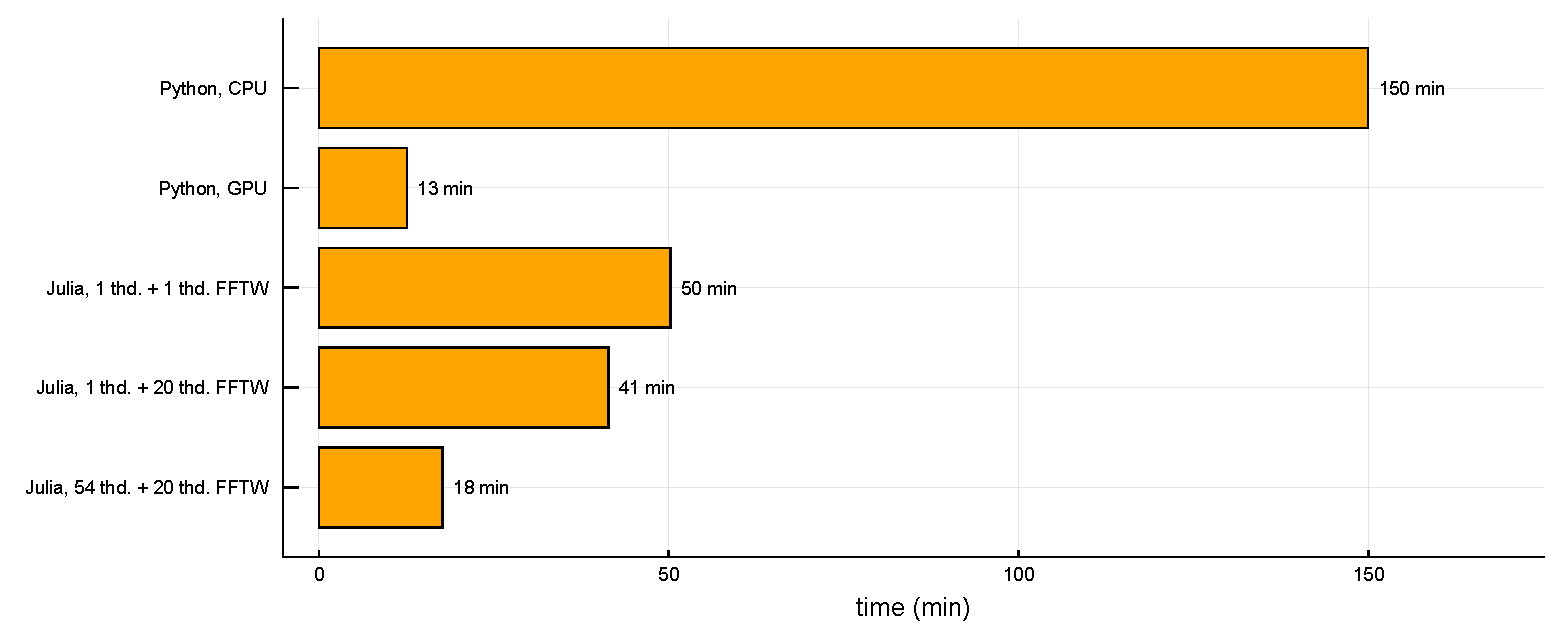
\includegraphics[width=\linewidth]{images/MSLR_recon_speed.pdf}
        \label{fig:MSLR_recon_speed}
    \end{minipage}
    \caption{asdf}
    \label{fig:3D_recon}
\end{figure}

\section{IRLS Implementation}

%\subsection{Description of Algorithm}
%\subsection{Implementation Details}

\begin{figure}
    \centering
    \begin{minipage}{0.48\linewidth}
        \centering
        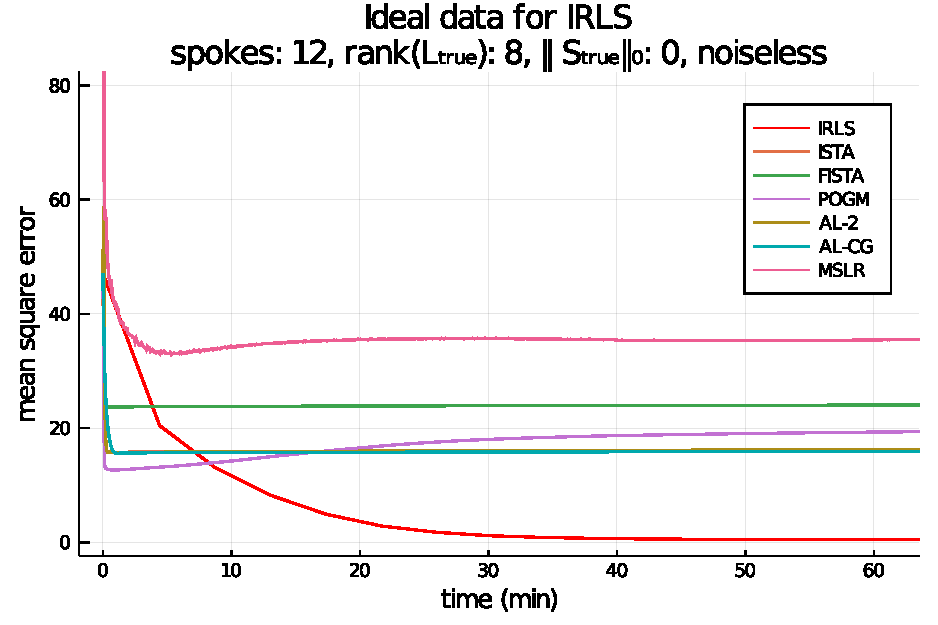
\includegraphics[width=\linewidth]{images/ideal_MSE.pdf}
        \label{fig:ideal_MSE}
    \end{minipage}
    \begin{minipage}{0.48\linewidth}
        \centering
        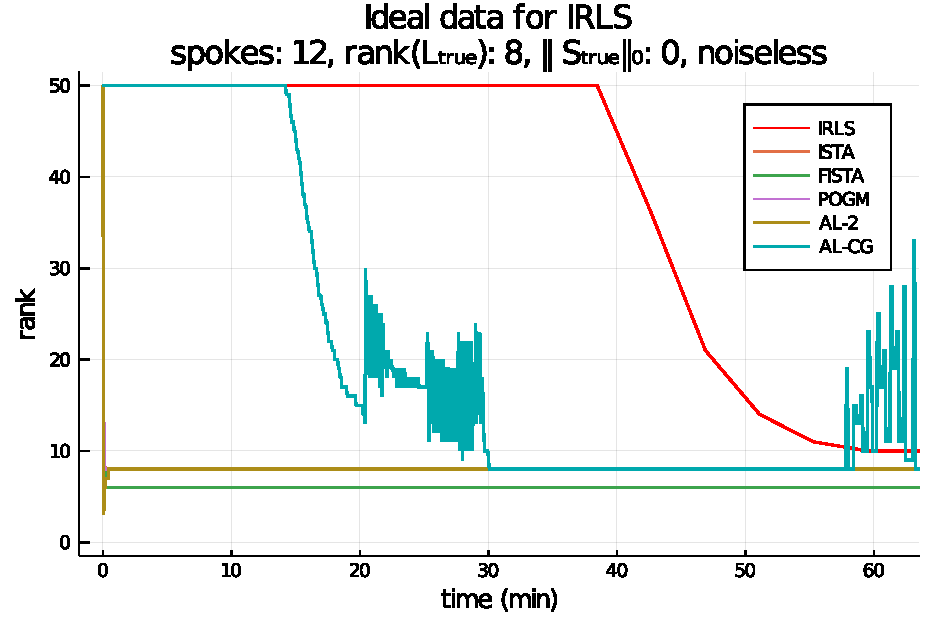
\includegraphics[width=\linewidth]{images/ideal_rank.pdf}
        \label{fig:ideal_rank}
    \end{minipage}
    \caption{asdf}
    \label{fig:ideal_recon}
\end{figure}

\begin{figure}
    \centering
    \begin{minipage}{0.48\linewidth}
        \centering
        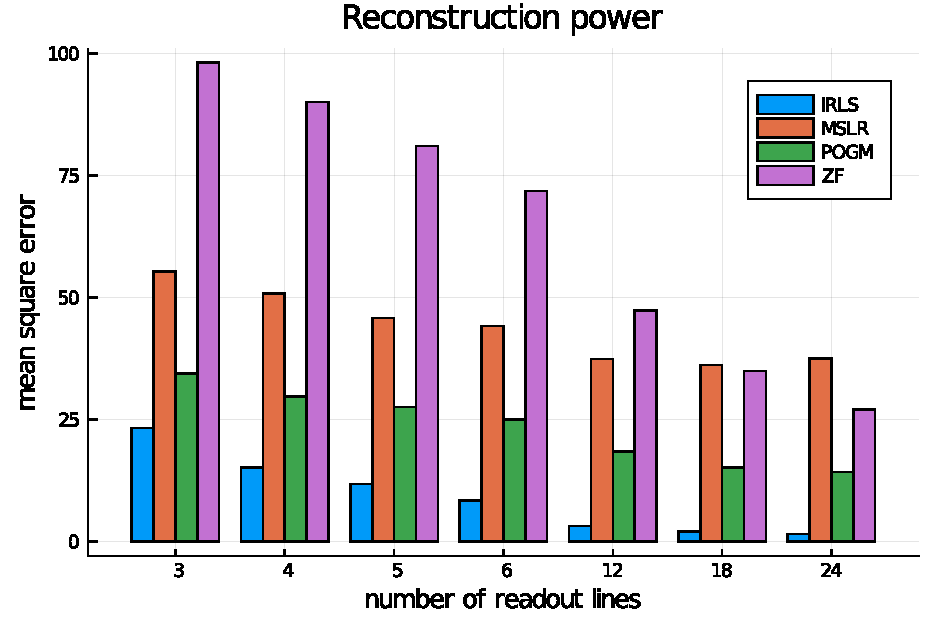
\includegraphics[width=\linewidth]{images/reconstruction_power.pdf}
        \label{fig:reconstruction_power}
    \end{minipage}
    \begin{minipage}{0.48\linewidth}
        \centering
        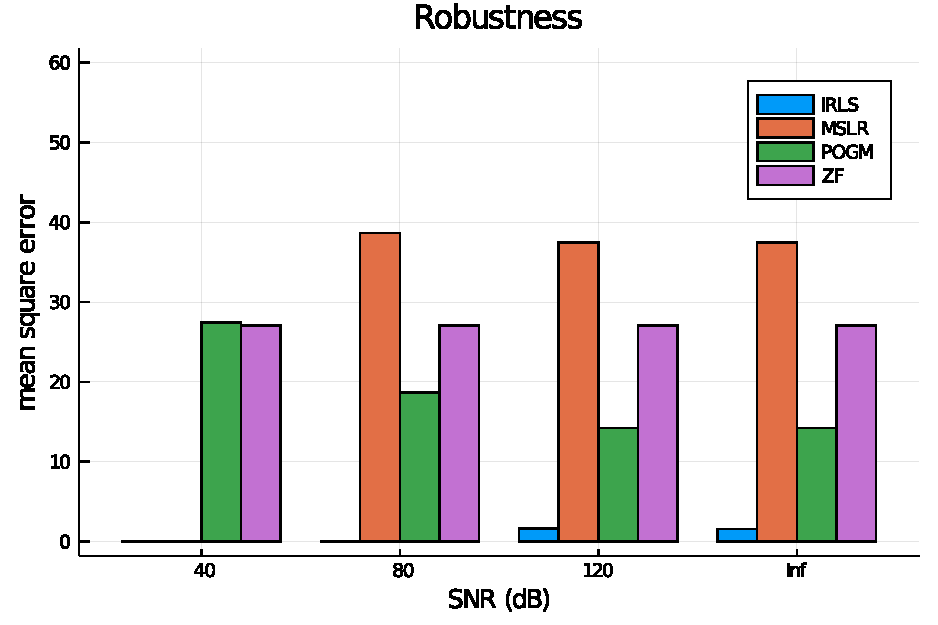
\includegraphics[width=\linewidth]{images/noise_tolerance.pdf}
        \label{fig:noise_tolerance}
    \end{minipage}
    \caption{asdf}
    \label{fig:IRLS_analysis}
\end{figure}

\begin{figure}
    \centering
    \begin{minipage}{0.48\linewidth}
        \centering
        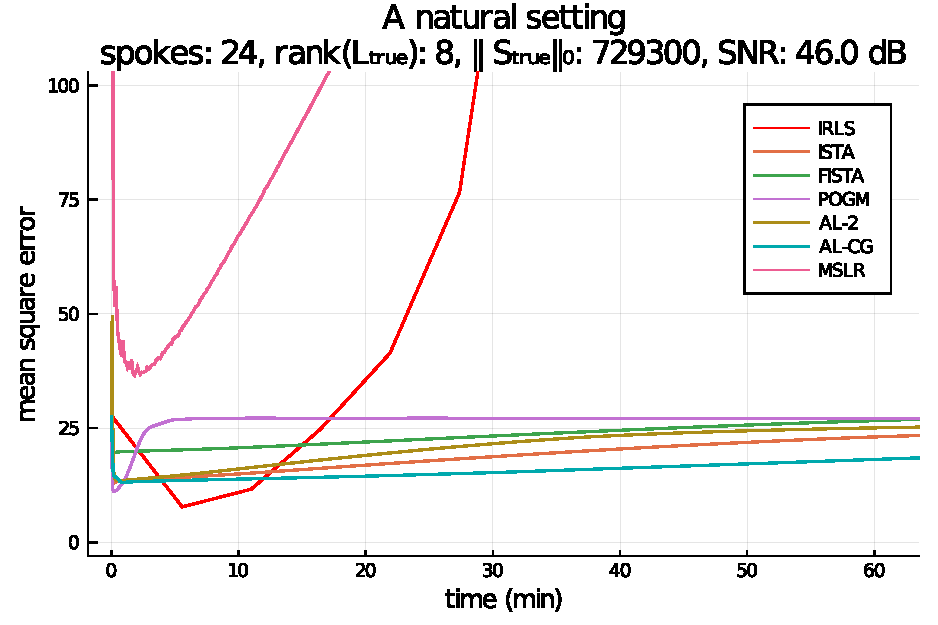
\includegraphics[width=\linewidth]{images/orig_MSE.pdf}
        \label{fig:orig_MSE}
    \end{minipage}
    \begin{minipage}{0.48\linewidth}
        \centering
        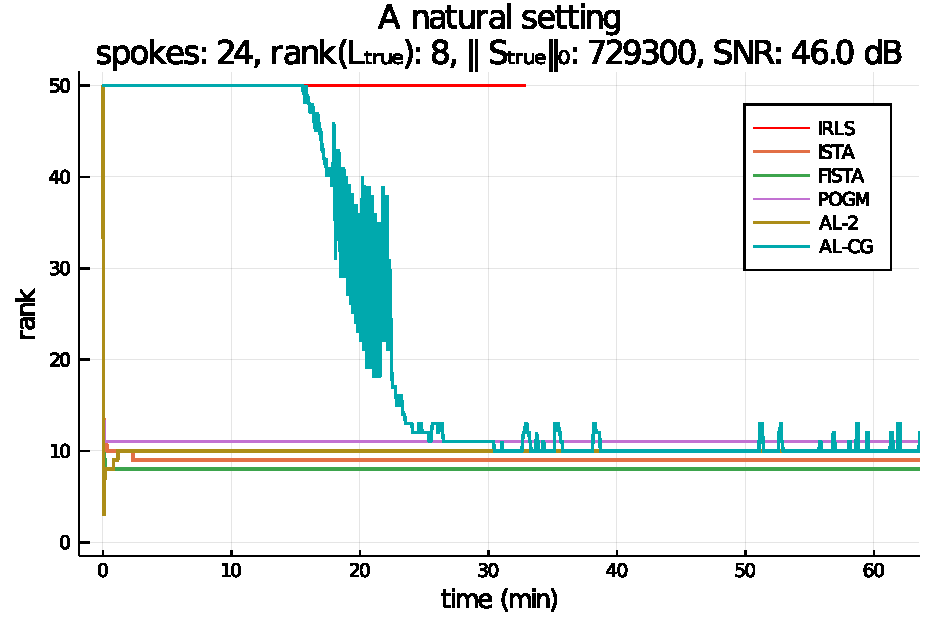
\includegraphics[width=\linewidth]{images/orig_rank.pdf}
        \label{fig:orig_rank}
    \end{minipage}
    \caption{asdf}
    \label{fig:orig}
\end{figure}

\begin{figure}
    \centering
    \begin{minipage}{0.48\linewidth}
        \centering
        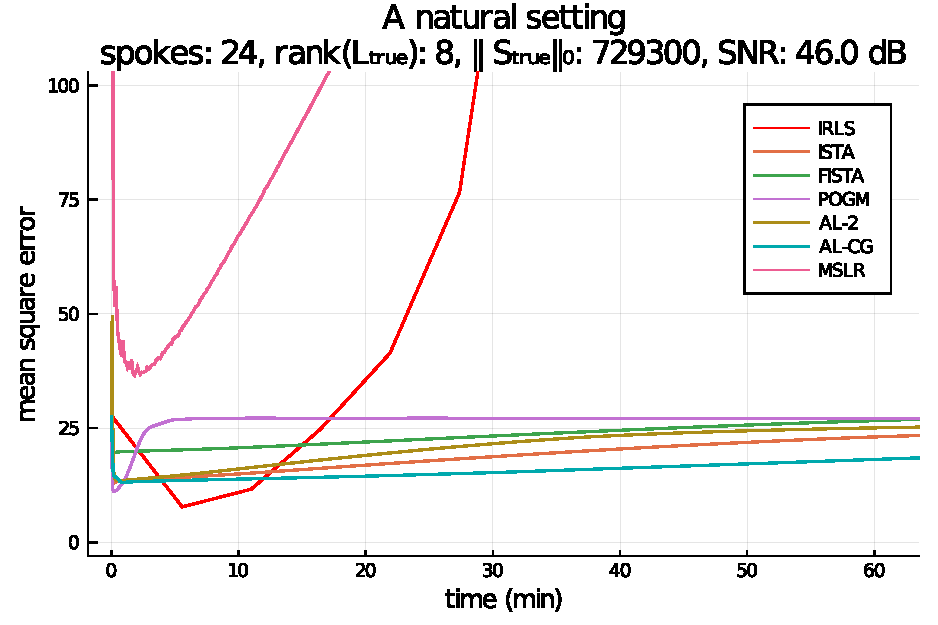
\includegraphics[width=\linewidth]{images/orig_MSE.pdf}
        \label{fig:orig_MSE}
    \end{minipage}
    \begin{minipage}{0.48\linewidth}
        \centering
        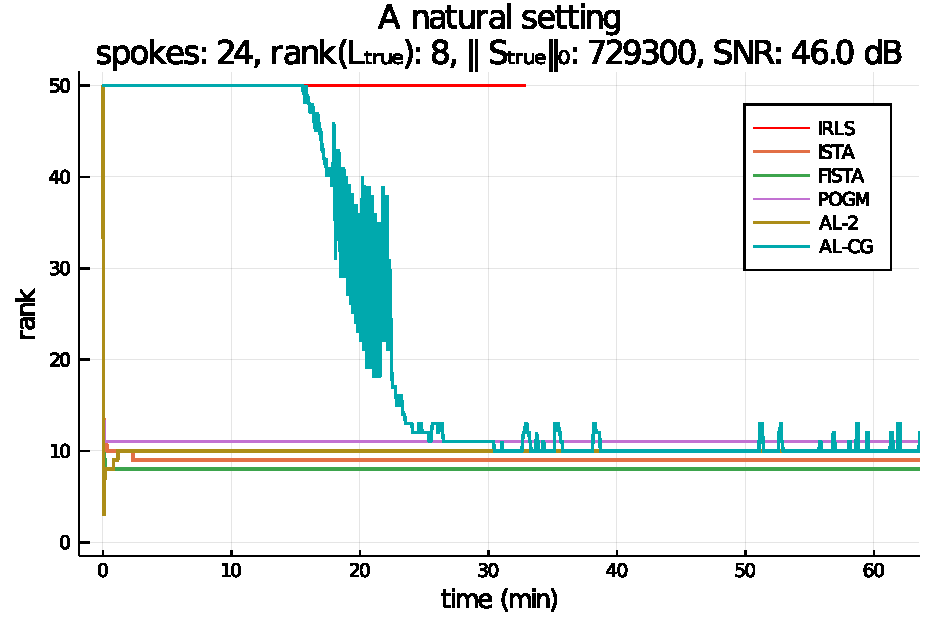
\includegraphics[width=\linewidth]{images/orig_rank.pdf}
        \label{fig:orig_rank}
    \end{minipage}
    \caption{asdf}
    \label{fig:orig}
\end{figure}

\begin{figure}
    \centering
    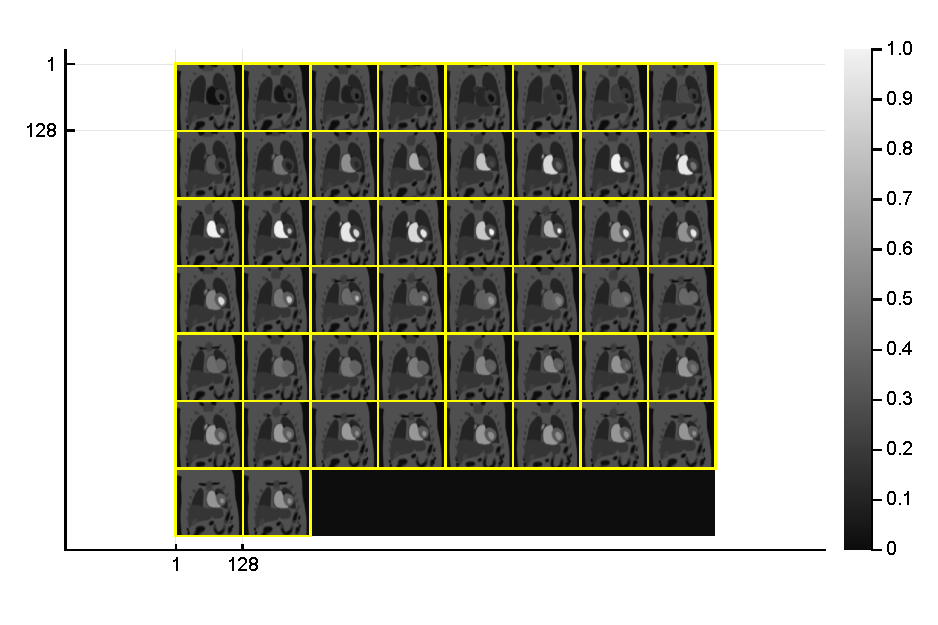
\includegraphics[width=0.46\linewidth]{images/PINCAT_all.pdf}
    \caption{Caption}
    \label{fig:PINCAT_all}
\end{figure}

\begin{figure}
    \centering
    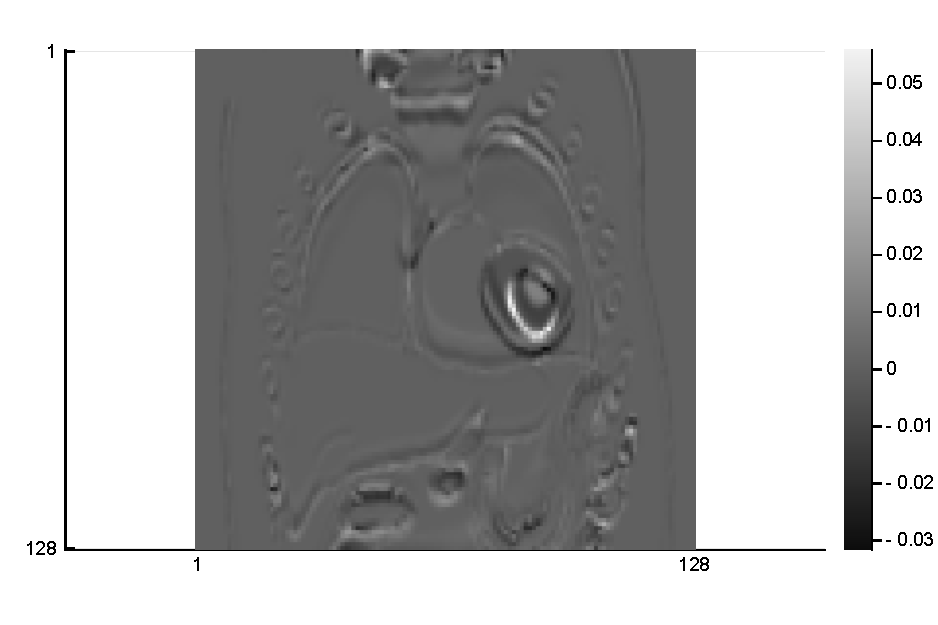
\includegraphics[width=0.46\linewidth]{images/PINCAT_diff_t20.pdf}
    \caption{Caption}
    \label{fig:PINCAT_diff_t20}
\end{figure}

\begin{figure}
    \centering
    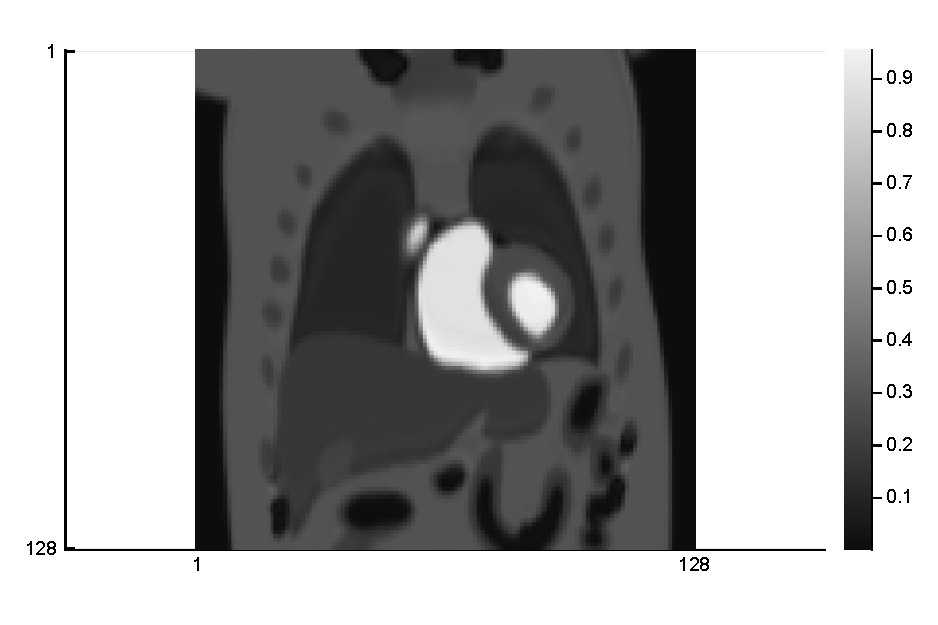
\includegraphics[width=0.46\linewidth]{images/PINCAT_IRLS_recon.pdf}
    \caption{Caption}
    \label{fig:PINCAT_IRLS_recon}
\end{figure}

\begin{figure}
    \centering
    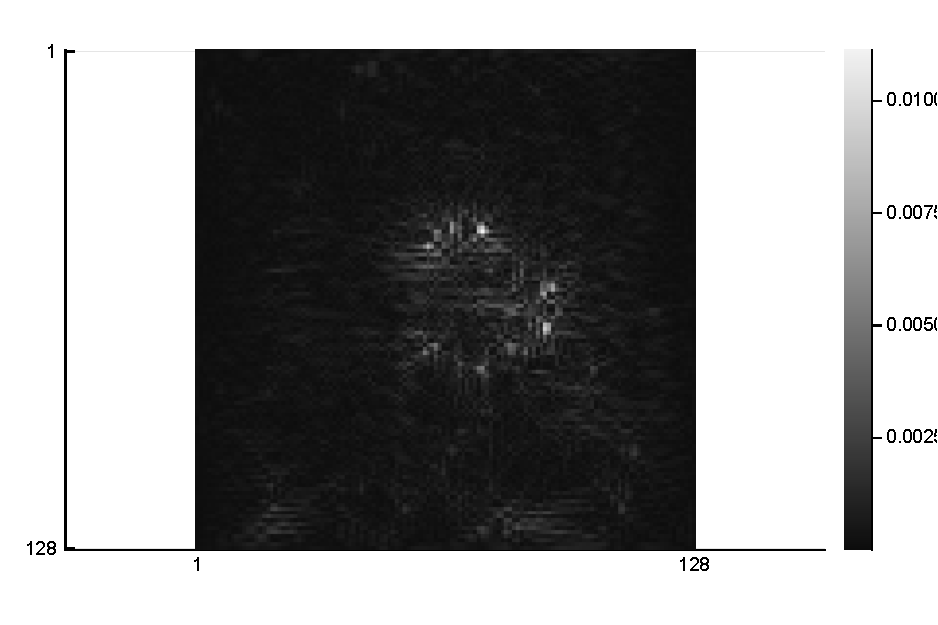
\includegraphics[width=0.46\linewidth]{images/PINCAT_IRLS_recon_error.pdf}
    \caption{Caption}
    \label{fig:PINCAT_IRLS_recon_error}
\end{figure}

\begin{figure}
    \centering
    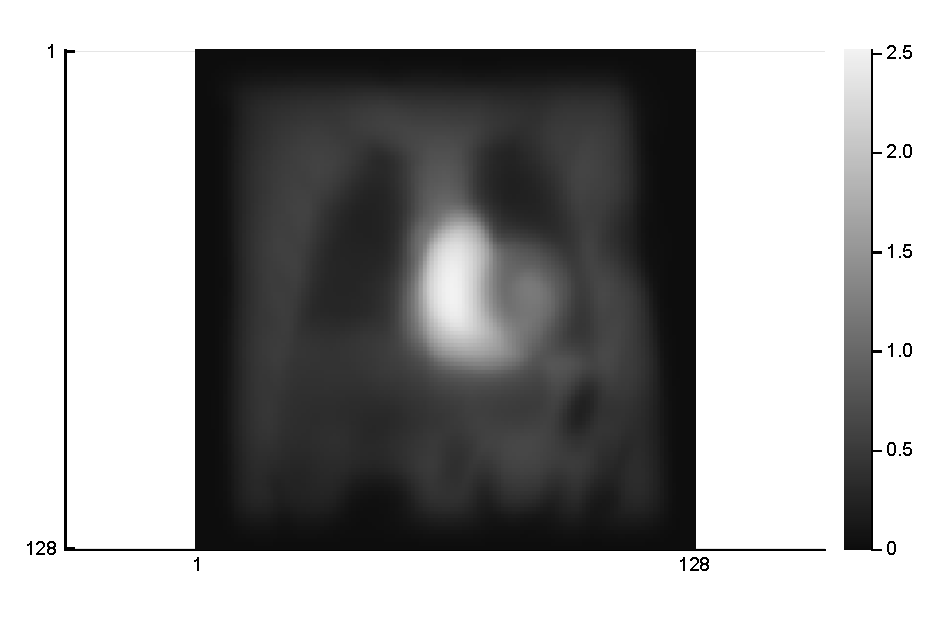
\includegraphics[width=0.46\linewidth]{images/PINCAT_MSLR_recon.pdf}
    \caption{Caption}
    \label{fig:PINCAT_MSLR_recon}
\end{figure}

\begin{figure}
    \centering
    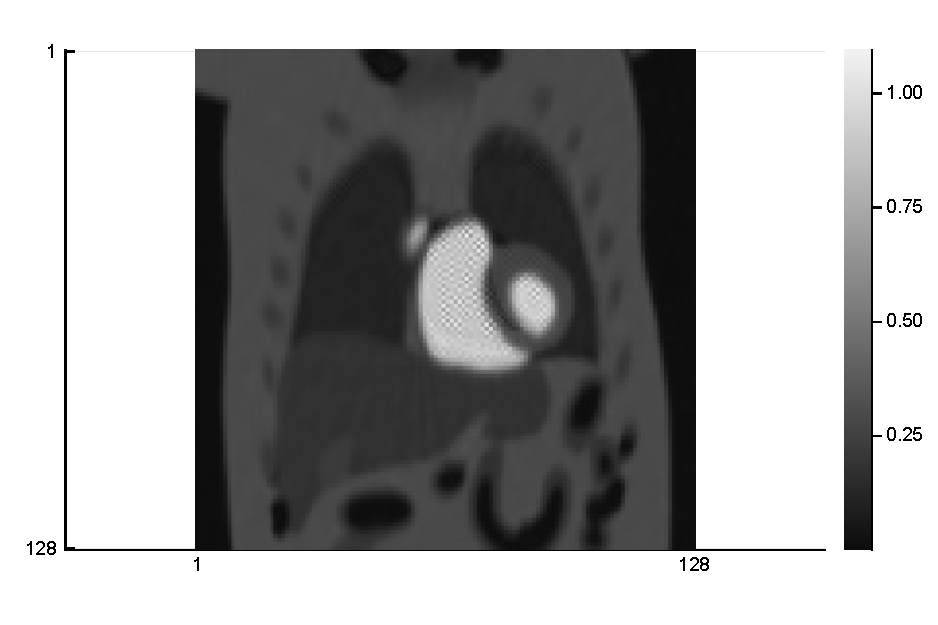
\includegraphics[width=0.46\linewidth]{images/PINCAT_POGM_recon.pdf}
    \caption{Caption}
    \label{fig:PINCAT_POGM_recon}
\end{figure}

\clearpage % You need \clearpage at the end of every chapter to force images included in this chapter to be rendered in somewhere else
